\documentclass[]{report}
\usepackage{graphicx}
\graphicspath{ {./images/} }
\usepackage{hyperref}
\hypersetup{
	colorlinks=true,
	linkcolor=blue,
	filecolor=magenta,      
	urlcolor=cyan,
}

% Title Page
\title{COVID-19 early days \\ \large A Multivariate Linear Regression and Decision Tree Analysis \\ Approach to understanding the early progression of the novel corona virus based on country demographics}

\author{Lindo Khoza \\ willkhoza@gmail.com}


\begin{document}
\maketitle

\begin{abstract}
This analysis is based on the \href{https://github.com/willkhoza/COVID_SA}{Novel Coronavirus (COVID-19) Cases from a South African perspective} repository \cite{covidsa}. The intention is to understand the influence of demographic variables on the early progression of the COVID-19 within different countries. As such, models used are chosen for their simplicity and transparency.

This report can only serve as a snapshot in time as the data process is live and unfolding. The diagrams and fitted models will change, this is captured in the repository. Alternatively, the annexure that accompanies the report is dynamically generated, and the plots and information reflected there is updated accordingly.

The repository sources data from the \href{https://github.com/CSSEGISandData/COVID-19}{2019 Novel Coronavirus COVID-19 (2019-nCoV) Data Repository by Johns Hopkins CSSE} repository \cite{jhu}.

The analysis shows that older populations have a tendency travel more, resulting in then having more exposure to COVID-19. This coupled with other pecks of being old, appears to have been a statistcally significant driver of the COVID-19 pandemic affecting older people with the extreme intensity which it has.

\end{abstract}

\section*{Background}

COVID-19 is an infectious disease caused by a variant of the coronavirus family. The disease is associated with respiratory illnesses.

The primary action taken by governments to curb the spread of the disease is to encourage people to wash hands frequently, to social distance, and to restrict overall physical interaction with other people.

\section{Variable Description}

\subsection{Response Variables}

The multivariate linear regression uses demographic predictor variables to model the following response variables:


\begin{enumerate}
	\item $t_1$: The number of days it takes for a country to report a confirmed infection following the earliest report date in china.
	\item $t_2$: The number of days it takes for a country to report it's first known death as a result of the virus following it's first confirmed infection.
\end{enumerate}

The earliest confirmed case  of COVID-19 is  unofficially reported to be 17 November 2019 \cite{scmp}.

\subsection{Demographic Predictors}
The following demographic variables are used to fit the model:

\begin{enumerate}
	\item Population: country population
	\item Annual Change: annual change of population in proportions
	\item Annual Change Absolute: annual change of population in absolute terms 
	\item Density: $P/km^2$
	\item Land Area: $km^2$
	\item Migrants: Net migration in the country
	\item Fertility Rate
	\item Median Age
	\item Urban Population: Proportion of population living in urban areas
	\item World Share
	\item Migration index =  $sgn$(Migrants)$\times ln$($abs$(Migrants))
	\item lnPopulation = $ln$(Population)
\end{enumerate}

The demographic data is with respect to the year 2020, as reported by \href{https://www.worldometers.info/world-population/population-by-country/}{worldometer} \cite{worldometer}.

\subsection{Additional Predictors}

An additional predictor was retrieved from  \href{https://en.wikipedia.org/wiki/List_of_countries_by_airline_passengers}{wikipedia} \cite{wikipedia} due to the association of the virus with travelling:

\begin{enumerate}
	
	\item Passengers: Annual number of airline passengers per country
	
	\item lnPassengers = $ln$(Passengers)
\end{enumerate}

The data has been processed and stored in the repository.


\section{Summary Statistics}

\subsection*{Overview}

Data from approximately 169 countries was used to fit the linear model. Atleast 54 of these countries have not recorded a death as a result of COVID-19. Also, atleast 11 countries have missing demographic data, especially countries with very small population sizes such the Holy See. 

\subsection*{Data Source Design}

In the JHU repository \cite{jhu}, data from 4 cruise ships was also observed from the original JHU repository, as such these data points will systematically not have demographic information. 

Furthermore, the data capturing period is from 22 January 2019 onwards, as such, countries which experience left truncation (China, Taiwan, South Korea, US, Japan, Thailand) are excluded from the model fitting dataset.

\newpage

\subsection*{Central Statistics}

\begin{table}[htb]
	\centering
	\caption{Response Variable Summary Statistics}
	\begin{tabular}{lllllll}
		& Min & $Q_1$ & $Q_2$ & $Q_3$ & Max & Mean  \\
		$t_1$ & 67  & 102   & 110   & 119   & 135 & 108.4 \\
		$t_2$ & 0   & 8     & 15    & 22    & 61  & 17.31
	\end{tabular}
\end{table}

\subsection*{Data Snippet}
\begin{table}[htb]
	\centering
	\caption{Snippet of data after preprocessing \cite{covidsa}}
	\label{snippet1}
	\begin{tabular}{llllll}
		Country      & $t_1$  & $t_2$ & inception  & confirmed  & death      \\
		Zimbabwe     & 124 & 3  & 17/11/2019 & 20/03/2020 & 23/03/2020 \\
		South Africa & 109 & 22 & 17/11/2019 & 05/03/2020 & 27/03/2020
	\end{tabular}
\end{table}

\newpage

\subsection{Dependence and Concordance}

\begin{enumerate}
	\item{$t_1 \sim t_2$}
	
	The pearson correlation between the 2 response variables is  $-0.78$. This shows that $t_1$ is inversely related to $t_2$, such that taking a long to report a first confirmed infection is associated with taking a short amount of time to report a death soon afterwards.
	
	For instance, the case of Zimbabwe and South Africa as shown in \ref{snippet1}. Zimbabwe 124 days to report a first case, only to report a death 3 days later. Where else South Africa took 109 days to report a first case, and reported a death after 22 days.
	
	Assuming the COVID-19 force of mortality to not be dependent on the time the first case is confirmed, it may appear that countries who take long to report instances of the virus are experiencing an oversight issue, such that by the time they commence their mortality investigation by reporting a first case, some COVID-19 lives are actually reaching the end on their lifetimes.
	
	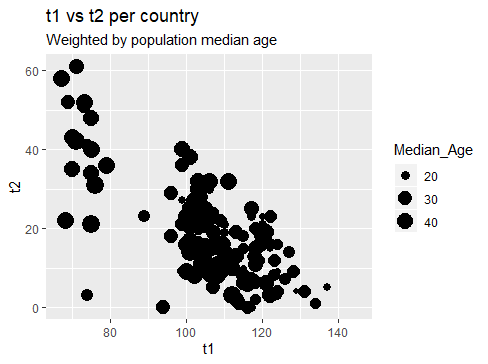
\includegraphics{t1vt2.png}
	
	\newpage
	
	\item{Passengers $\sim t_1$}
	
	The pearson correlation between Population and $t_1$ is $-0.565$. This shows that $t_1$ is also inversely related to the number of airline passengers, such that a large number number of airline passengers is associated with reporting a first confirmed case sooner. 
	
	Furthermore, we observe that $ln$(Passengers) axis separates the $t_1$ into axis into 2 categories, i.e. The segment below 12 and the segment above 12. These identify countries with low and high numbers of air passengers respectively, with a strange realization that countries with low numbers of air passengers tend to have higher fertility rates. This narative is further reinforced by the next relationship, which shows that countries with a low number of airpassengers, tend to have younger populations.
	
	i.e: Older populations have a tendency travel more (resulting in more exposure to COVID-19) compared to younger populations, they also have more interaction with other networks of older people. This, coupled with having weaker immune systems, may have been a major driver of the COVID-19 pandemic affecting older people with the extreme intensity which it has.
	
	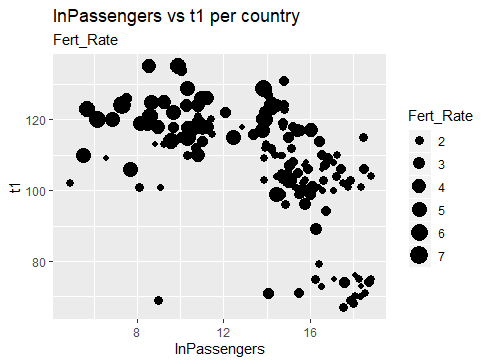
\includegraphics{lnpvt1.png}
	
	\newpage
	
	\item{Median Age $\sim t_1$}
	
	The pearson correlation is $-0.45$.
	
	To reiterate, older people appear to travel more, and even those who may not travel are more likely to interact with older people who do as opposed to their young counter parts. This, coupled with them having weaker immune systems, appears to be one of the drivers of networks of old people being exposed and harshly affected by the virus. 
	
	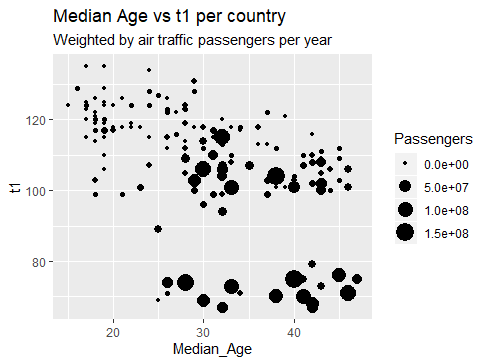
\includegraphics{mavt1.png}
	
	\newpage
	
	\item $. \sim .$ (correlogram)
	
	For completeness, see below correlogram for summary of all other relationships with respect to the pearson correlation.
	 
	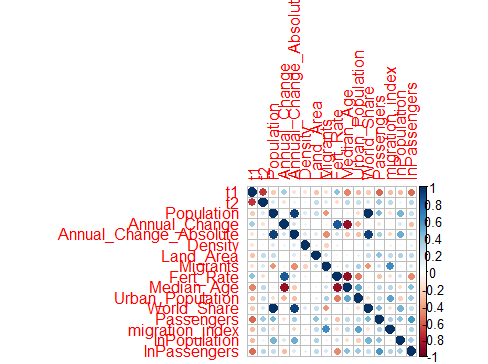
\includegraphics{corr.png}
\end{enumerate}

\newpage
\section{$t_1$: Decision Tree}

The following decision tree model was fitted for variable $t_1$

\begin{figure}[htb]
	\centering
	\caption{Decision Tree model for $t_1$ with complexity parameter of 0.025 }
	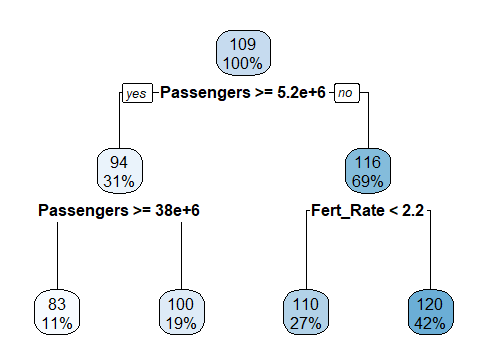
\includegraphics{tree.png}
\end{figure}


The decision tree re-iterates the theory that older people tend to travel, and as a result have more exposure to COVID-19 as opposed to their younger counter parts. 

The model begins by identifying that countries with a large number of air travellers are the purest segment to identify the countries with the lowest time to report a first case. It further segments countries who have less fertility rates and annual growth rates as those who take the least time to report a first case. Both these cases point out to older populations, who are not as fertile, but have the means to use air travel frequently.

\newpage

\section{$t_2$: Multivariate Linear Regression}

The following stepwise multivariate linear regression model was fitted for variable $t_2$

$$t_2 = 118.61624 -0.72402 t_1 - 0.21348 X_{Median Age} -1.14529 X_{lnPopulation}$$

It produces an $R^2$ of 0.626, which means the linear model accounts for approximately 62.6\% of the variation in $t_2$. This will suffice for the purposes of this report.

The linear model uses $t_1$, Median Age, and $ln$(Population) to explain $t_2$. Such that an increase in any one of these predictors is expected to reduce the amount of time it takes to observe the first death.

All other predictors have been found to not be statistically significant in accordance to the stepwise procedure based on the AIC criterion.


\begin{thebibliography}{9}
	\bibitem{scmp} 
	Ma Josephina 
	\textit{China's first confirmed Covid-19 case traced back to November 17}. 
	South China Morning Post, 13 March 2020.
	\\\texttt{https://www.scmp.com/news/china/society/article/3074991/coronavirus-chinas-first-confirmed-covid-19-case-traced-back}
	
	\bibitem{wikipedia} 
	List of countries by airline passengers
	\\\texttt{https://en.wikipedia.org/wiki/List\_of\_countries\_by\_airline\_passengers}
	
	\bibitem{worldometer}
	Countries in the world by population (2020)
	\\\texttt{https://www.worldometers.info/world-population/population-by-country/}
	
	\bibitem{jhu}
	2019 Novel Coronavirus COVID-19 (2019-nCoV) Data Repository by Johns Hopkins CSSE
	\\\texttt{https://github.com/CSSEGISandData/COVID-19}
	
	\bibitem{covidsa}
	Lindo Khoza
	\textit{Novel Coronavirus (COVID-19) Cases from a South African perspective}
	\\\texttt{https://github.com/willkhoza/COVID\_SA}
	
\end{thebibliography}

\end{document}          
